\documentclass{article}

%% doc settings
\hyphenchar\font=-1 % suppress hyphenation
\setlength\parindent{0pt} % suppress indentation
\usepackage[margin=1.5truein]{geometry} % set page margins

%% core libraries
\usepackage{listings}
\usepackage{fancyhdr}
\usepackage{lastpage}
\usepackage{url}
\usepackage{xcolor}
\usepackage{hyperref}
\usepackage{natbib}
\usepackage{tikz}

%% sec libraries
\usetikzlibrary{shapes,arrows}
\usepackage{textcomp}

%% link viz
\hypersetup{
    colorlinks = true,
    linkcolor = red,
    urlcolor = red,
    citecolor = black
}

%% page nums
\pagestyle{fancy}
\fancyhf{}
\fancyfoot[C]{Pg. \thepage \space of \pageref*{LastPage}}
\renewcommand{\headrulewidth}{0pt}

%% begin doc
\begin{document}
\title{SYSEN 6150: Model Based Systems Engineering\\~\\
    \Large Context Diagrams \& Errors
}
\author{
    Nick Kunz [NetID: \url{nhk37}] \hyperlink{nhk37@cornell.edu}{nhk37@cornell.edu}}
\date{September 12, 2022}
\maketitle
\thispagestyle{fancy}

\section*{Context Diagram: Public Transit Prediction System}

%% diagram style
\tikzset{
    block/.style    = {draw, thick, rectangle, minimum height = 3em, minimum width = 3em},
    input/.style    = {coordinate},
    output/.style   = {coordinate}
}

%% drawing
\begin{tikzpicture}[auto, thick, node distance=2cm, >=triangle 45]

%% system node
\draw node at (6,-4) [block, name=system]{Prediction System};
\draw [color=black, dashed](2,-6) rectangle (10,-2);

%% context nodes
\draw node at (0,0) [block, name=context1]{Data};
\draw node at (-0.5,-0.55) [output, name=output1a]{};
\draw node at (0.5,-0.55) [output, name=output1b]{};

\draw node at (6,0) [block, name=context2]{Servers};

\draw node at (12,0) [block, name=context3]{Interfaces};
\draw node at (11.15,-0.5) [output, name=output3]{};

\draw node at (0,-8) [block, name=context4]{Vehicles};
\draw node at (-0.5,-7.5) [output, name=output4a]{};
\draw node at (0,-8.55) [output, name=output4b]{};
\draw node at (0,-9) [output, name=output4c]{};

\draw node at (6,-8) [block, name=context5]{Passengers};
\draw node at (6.95,-7.5) [output, name=output5]{};

\draw node at (12,-8) [block, name=context6]{Drivers};
\draw node at (11.15,-7.5) [output, name=output6a]{};
\draw node at (12,-8.55) [output, name=output6b]{};
\draw node at (12,-9) [output, name=output6c]{};

\draw node at (3,0) [block, name=context7]{Storage};
\draw node at (9,0) [block, name=context8]{Balancers};

%% edges of system
\draw[-] (system) -| node {}(output1b);
\draw[-] (system) -| node {}(context7);
\draw[-] (system) -- node {}(context2);
\draw[-] (system) -| node {}(context6);

%% edges of context
\draw[-] (context1) -- node {}(context7);
\draw[-] (context7) -- node {}(context2);
\draw[-] (context2) -- node {}(context8);
\draw[-] (context8) -- node {}(context3);

\draw[-] (context3) -- node {}(context6);
\draw[-] (output3) -- node {}(output6a);

\draw[-] (output6a) -- node {}(output5);
\draw[-] (output4a) -- node {}(output1a);
\draw[-] (output4b) -- node {}(output4c);

\draw[-] (context4) -- node {}(context5);
\draw[-] (context5) -- node {}(context6);
\draw[-] (output6b) -- node {}(output6c);
\draw[-] (output4c) -- node {}(output6c);

%% domain nodes
\draw [color=black, dotted](-1, 1.5) rectangle (13.25,-1);
\draw [color=black, dotted](-1, -10) rectangle (13.25,-7);

%% domain labels
\node at (-0.9, 0.5) [above=5mm, right=0mm]{\textsc{Computational Layer: Application Services (Enabling System)}};
\node at (-0.9,-10) [above=5mm, right=0mm]{\textsc{Physical Layer: Public Transit (Enabling System)}};
\node at (2.1,-6) [above=5mm, right=0mm]{\textsc{System of Interest}};

%% edge labels, compute layer
\node at (-0.55,-7.75) [above=5mm, right=0mm]{\footnotesize telemetry};
\node at (-0.55,-1.25) [above=5mm, right=0mm]{\footnotesize cache};
\node at (0.5,-1.25) [above=5mm, right=0mm]{\footnotesize send};
\node at (0.5,-0.25) [above=5mm, right=0mm]{\footnotesize send};
\node at (3,-1.25) [above=5mm, right=0mm]{\footnotesize send};
\node at (3.65,-0.25) [above=5mm, right=0mm]{\footnotesize send};
\node at (1.2,-0.75) [above=5mm, right=0mm]{\footnotesize persist};
\node at (4.15,-0.75) [above=5mm, right=0mm]{\footnotesize request};
\node at (3,-4.30) [above=5mm, right=0mm]{\footnotesize request};
\node at (6,-3.75) [above=5mm, right=0mm]{\footnotesize serve};
\node at (7.5,-4.3) [above=5mm, right=0mm]{\footnotesize make predictions};
\node at (6,-1.25) [above=5mm, right=0mm]{\footnotesize request};
\node at (6.65,-0.25) [above=5mm, right=0mm]{\footnotesize serve};
\node at (9.8,-0.25) [above=5mm, right=0mm]{\footnotesize throttle};
\node at (7,-0.75) [above=5mm, right=0mm]{\footnotesize request};
\node at (10.4,-0.75) [above=5mm, right=0mm]{\footnotesize load};
\node at (11.15,-1.25) [above=5mm, right=0mm]{\footnotesize send};
\node at (12,-1.25) [above=5mm, right=0mm]{\footnotesize send};

%% edge labels, physic layer
\node at (12,-7.75) [above=5mm, right=0mm]{\footnotesize request};
\node at (6.9,-7.75) [above=5mm, right=0mm]{\footnotesize request predictions};
\node at (6.9,-8.25) [above=5mm, right=0mm]{\footnotesize request service};
\node at (9.1,-8.75) [above=5mm, right=0mm]{\footnotesize provide service};
\node at (0.75,-8.25) [above=5mm, right=0mm]{\footnotesize transport};
\node at (4.3,-8.25) [above=5mm, right=0mm]{\footnotesize ride};
\node at (11.1,-9.3) [above=5mm, right=0mm]{\footnotesize drive};
\node at (0,-9.3) [above=5mm, right=0mm]{\footnotesize controlled by};

\end{tikzpicture}

\newpage
\section*{Context Diagram: Bad Practice}
\begin{figure}[htp]
    \centering
    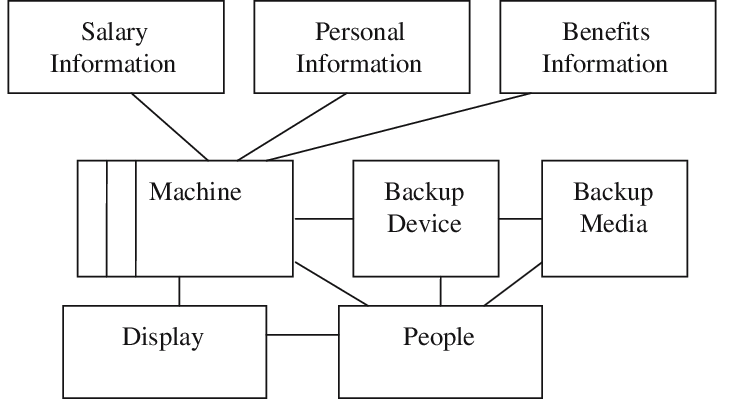
\includegraphics[width=9cm]{bad-exp.png}
    \caption{Example Context Diagram from \textit{"Using Trust Assumptions with Security Requirements"} by Haley, et. al.\cite{Haley}}
    \label{fig:bad}
\end{figure}

There are several ways in which the context diagram exhibited above could improve. Below are 3 techniques that could be utilized to help bring clarity to the diagram:
\begin{enumerate}
    \item Include a system boundary. In the example above, no system boundary was illustrated. A dashed box around the System of Interest (SOI) would bring focus to both the SOI, as well as the contextual components.
    \item Include line labels. Brief descriptors or verbs to denote the relationships between components, as well as statements within the system boundary to indicate how the contextual components relate to the SOI.
    \item Maintain a consistent component format. There is one example here where the\\ \textit{"Machine"} component contains additional lines intersecting the component box. Even if this could be substantiated, it is prudent to keep all of them the same appearance.
\end{enumerate}

%% ref sec
\newpage
\bibliographystyle{ieeetr}
\bibliography{ref.bib}

\end{document}